\chapter{Design}

Designing this system could take two different paths in order to create a directory tree representing the database. The first is to have a program look for changes in both the database and filesystem and then mirrors the changes from each to the other. The second method is to write a filesystem that is constantly being called with callbacks when the user performs an action such as creating a folder or deleting a file.

\section{Polling or Filesystem?}

\subsection{Polling}

This program would then be run at a regular interval to give the illusion that they were directly linked. There are numerous problems with this implementation with the most prominent being detecting the changes made on each side. Not all database management systems allow for the placement of triggers or streaming of incoming data to another source. The other side is simpler as there are already methods of looking for updated files in the form of modification dates and operating system APIs for registering for callbacks of changes such as \texttt{inotify} for Linux and \texttt{fs-events} for Mac OS X.

% TODO: More

\subsection{Filesystem}

By using a filesystem instead of an seperate polling program we tighten the feedback loop from changes to the files to the database. By doing this we avoid the potentially expensive operations of scanning the filesystem for changes and have direct callbacks that reference the exact file changed.

\section{Scaling Issues}

There is some concern about how this will scale up to the sizes that databases can reach. There are some unknowns such as how a filesystem will perform once it has millions of files in it, each representing a record in the database. Since users demand that a filesystem is responsive then a non-functional requirement should be made that the database returns all queries in a responsive manner. There are numerous ways that this could be done such as simple caching of values outside the database all the way up to using previous usage patterns to scan across the data on the disk in order to load it into memory before the query is ever made to creating useful indexes automatically to help regularly slow queries. However, it is unwise to spend unnecessary time considering solutions to problems that may not occur.

\section{The Querying Problem}

A database has 3 main duties when it comes to presenting the user with data: querying, updating and deleting. Our current solution to the problem provides a good solution to updating and deleting records but querying the database beyond basic operations is not easy to do with the limited actions avaliable to the filesystem.

In order to allow the user to perform more complex queries on the database a seperate application is needed. However it is critical that still presents the database as a filesystem. If we look at how users perform complex sequences of operations on a filesystem currently then there are two different approaches depending on the level of expertise of the user.

\subsection{Mirroring Filesystem Solutions}

If we have a task that we would like to perform such as resizing all of the images in a folder that were taken in the last week and which have ``flower'' in the filename then depending on the level of expertise of the user then they will probably approach it in two different ways.

A technical user will probably write a shell script or use multiple commands piped together to achieve the intended effect. A command such as the following will perform the above task:

\begin{verbatim}
  find . -type f -name "*.jpg" |
    grep "flower" |
    xargs convert -resize 50%
\end{verbatim}

Instead of performing the action in one step the user splits up the command into 3 logical steps of find the picures, filter the ones with flower in the name, and finally perform the resizing.

A non-technical user has a number of avaliable operations to them. The most widely used among Macintosh users is probably a program called Automator which is bundled with the operating system. It allows the user to do a similar thing to shell scripts by composing a workflow of similar duties to the programs above.

\begin{figure}[ht!]
	\centering
	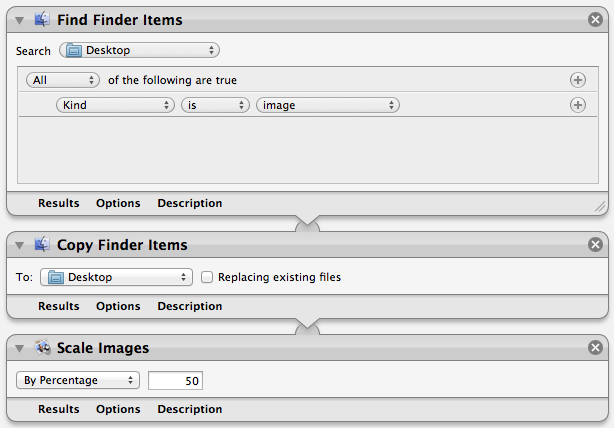
\includegraphics[width=0.9\textwidth]{images/automator}
	\caption{Automator Workflow}
	\label{fig:automator}
\end{figure}

\section{Creating SQL}